\chapter{Challanges of Microservices Architecture}\label{chapter:challanges_of_microservices_architecture}
This chapter focuses on various challenges faced while implementing microservices. In Section \ref{section:challanges_of_microservices_architecture/introduction}, various advantages of microservices along with its challenges are listed. Then each challenge is broken down into several sub-challenges and discussed further after Section \ref{section:challanges_of_microservices_architecture/integration}. For each challenges, various techniques which can be used to handle them are also presented. Again, in order to provide benefit from industry experience, the techniques used by SAP Hybris are also presented.
\section{Introduction}\label{section:challanges_of_microservices_architecture/introduction}
The Section \ref{subsection:context/monolith-disadvantages} lists some drawbacks of monolithic architecture and these have become the motivation for adopting microservices architecture. Microservices offer opportunities in various aspects however it can also be tricky to utilize them properly. It does come with few challanges. The response from Interview Question \ref{question:hybris_architecture/interview/question_1.5} also highlights some prominent challanges. In this chapter, the challanges of microservices alongside its advantages will be discussed. \cite{Fowler:2015aa}

\label{section:challanges_of_microservices_architecture/introduction/challenges}
  \begin{multicols}{2}
  \textbf{\underline{Advantages}} 
  \vfill
  \columnbreak
  \textbf{\underline{Challanges}}
  \end{multicols}
  \begin{multicols}{2}
  \textbf{Strong Modular Boundaries} \\It is not totally true that monolith have weaker modular structure than microservices but it is also not false to say that as the system gets bigger, it is very easy for monolith to turn into a big ball of mud. However, it is very difficult to do the same with microservices. Each microservice is a cohesive unit with full control upon its business entities. The only way to access its data is through its \acrshort{API}.
  \vfill
  \columnbreak
  \textbf{Distributed System Complexity} \\The infrastructure of microservices is distributed, which brings many complications alongside, as listed by 8 fallacies.\cite{Factor:2014aa} The calls are remote which are imminent to accomplish business goals. The remote calls are slower than local and affect performance to a great deal. Additionally, network is not reliable which makes it challenging to handle failures.
  \end{multicols}

\begin{multicols}{2}
  \textbf{Independent Deployment} \\Due the nature of microservices being autonomous components, each microservice can be deployed independently. Deployment of microservices is thus easy compared to monolith application where a small change needs the whole system to be deployed.\cite{Newman:2015aa}
  \vfill
  \columnbreak
  \textbf{Integration} \\It is challanging to prevent breaking other microservices when deploying a service. Similarly, as each microservice has its own data, the collaboration among microservices and sharing of data can be complex.
   \end{multicols}
   
  \begin{multicols}{2}
  \textbf{Agile}\\ Each microservice is focused to single responsibility, changes are easy to implement. At the same time, as the microservices are autonomous, they can be deployed independently, decreasing the release cycle time.
  \vfill
  \columnbreak
  \textbf{Operational Complexity} \\ As the number of microservices increases, it becomes difficult to deploy in an acceptable speed and becomes more complicated as the frequency of changes increase. Similary, as the granularity of microservices decreases, the number of microservices increases which shifts the complexity towards the interconnections. Ultimately, it becomes complex to monitor and debug microservices.
   \end{multicols}
\\
In the following sections of this chapter, various ways to tackle the challenges mentioned in Section \ref{section:challanges_of_microservices_architecture/introduction/challenges} are discussed in detail.

\section{Integration}\label{section:challanges_of_microservices_architecture/integration}
The collaboration among various microservices whilst maintaining autonomous deployment is challenging. In this section, various challanges associated with integration and their potential remedies are discussed.

\subsection{Sharing Data}\label{section:challanges_of_microservices_architecture/integration/sharing_data}
An easiest way to collaborate is to allow services to access and update a common datasource. However, using this kind of integration creates various problems.\cite{Newman:2015aa}\\
\textbf{Problems}\label{section:challanges_of_microservices_architecture/integration/problems}
\begin{enumerate}
\item The shared database acts as a point of coupling among the collaborating microservices. If a microservice make any changes to its data schema, there is high probability that other services would need to be changed as well. Loose Coupling is compromised.
\item The business logic related to the shared data may be spread across multiple services. Changing the business logic is difficult. Cohesion is compromised.
\item Multiple services are tied to a single database technology. Migrating to a different technology at any point is hard.
\end{enumerate}
\\
\\
\textbf{Alternatives}\label{section:challanges_of_microservices_architecture/integration/alternatives}
\\
There are three distinct alternatives.\cite{Richardson:2015aa}
\begin{enumerate}
\item \textbf{private tables per service} - multiple services share same database underneath but each service owns a set of tables.
\item \textbf{schema per service} - multiple services share same database however each service owns its own database schema.
\item \textbf{database server per service} - each service has a dedicated database server underneath.
\end{enumerate}
\\
\begin{shaded}Techniques\end{shaded}\label{section:challanges_of_microservices_architecture/integration/sharing_data/techniques}
\\
The logical separation of data among services discussed in the Section \ref{section:challanges_of_microservices_architecture/integration/alternatives} increases autonomy but also make it difficult to access and create consistent view of data. However these can be compensated using following approaches.\cite{Richardson:2016aa} \cite{Richardson:2015aa}
\begin{enumerate}
\item The implementation of business transaction which spans multiple services is difficult and not recommended because of \acrshort{CAP} Theorem \ref{section:appendices/CAP_theorem}. The solution is to apply eventual consistency \ref{section:appendices/eventual_consistency} focussing more on availability.
\item The implementation of queries to join data from multiple databases can be complicated. There are two alternatives to achieve this.
    \begin{enumerate}
        \item A separate mashup service can be used to handle the logic to join data from multiple services by accessing respective \acrshort{API}s.
        \item \acrshort{CQRS} pattern \ref{section:appendices/CQRS} can be used by maintaining separate views as well as logic for updating and querying data.
    \end{enumerate}
\item The need for sharing data among various autonomous services cannot be avoided completely. It can be achieved by one of the following approaches.
    \begin{enumerate}
        \item The data can be directly accessed by using the resource owner's \acrshort{API}.
        \item The required data can be duplicated into another service and made consistent with the owner's data using event driven approach.
    \end{enumerate}
\end{enumerate}
\begin{shaded}
SAP Hybris uses the technique of maintaining private schema per microservice as listed in the Section \ref{section:challanges_of_microservices_architecture/integration/alternatives} in order to share data. For this purpose, there is a generic microservice called "Document" which handles the task of managing data for all microservices per each tenant and application. Furthermore, SAP Hybris follows eventual consistency and creates various mashup services for collective view of data from multiple services. Additionally, either data are duplicated to decrease the network overload or when fresh data is required, resource owner's \acrshort{API} is accessed directly.
\end{shaded}

\subsection{Inter-Service Communication}\label{section:challanges_of_microservices_architecture/integration/inter_service_communication}
It is correct that a microservice is an autonomous component but the necessity of interaction among microservices cannot be denied as well. The various possible interactions among microservices is shown in Figure \ref{fig:challanges_of_microservices_architecture/integration/inter_service_communication/interaction_styles_among_microservices}.\cite{Richardson:2015ab}
\begin{figure}[H]
\begin{center}
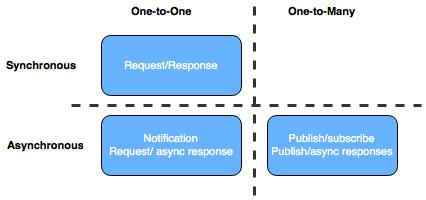
\includegraphics[width=0.8\textwidth]{figures/challenges_one_interaction_styles}
\caption{Inteaction Styles among microservices [\cite{Richardson:2015ab}]}
\label{fig:challanges_of_microservices_architecture/integration/inter_service_communication/interaction_styles_among_microservices}
\end{center}
\end{figure}
\\
\\
\textbf{One to One interactions}
\\
\begin{enumerate}
\item \textbf{Request/Response}: It is synchronous interaction where client sends request and expects for response from server.
\item \textbf{Notification}: It is asynchronous one way interaction where cliend sends request but no reply is sent from server.
\item \textbf{Request/async Response}: It is asynchronous interaction where client requests server but does not block waiting for response. The server send response asynchronously.
\end{enumerate}
\\
\\
\textbf{One to Many interactions}
\\
\begin{enumerate}
\item \textbf{Publish/subscribe}: A service publishes notification which is consumed by other interested services.
\item \textbf{Publish/async responses}: A service publishes request which is consumed by interested services. The services then send asynchronous responses.
\end{enumerate}
\\
\\

\begin{shaded}Techniques\end{shaded}
\subsubsection{Synchronous and Asynchronous}\label{section:challanges_of_microservices_architecture/integration/synchronous_and_asynchronous}
Each of the interactions listed in Section \ref{section:challanges_of_microservices_architecture/integration/inter_service_communication} has its own place in an application. An application can contain a mixture of these interactions. However, a clear idea about the requirement as well as thorough knowledge regarding drawbacks associated with each interaction is necessary before a decision can be made which one to choose for a specific case.\cite{Newman:2015aa}\cite{Richardson:2014aa}\cite{Morris:2015aa}\\
\textbf{Synchronous Interaction}
\\
It is simple to understand the flow and natural way of implementing an interaction. However, as the volume of interactions get higher and distributes to various levels, it increases the overal blocking period of client and thus increases latency. The synchronous nature of interaction increases temporal coupling between services which demands both to be active at the same time. Since, the synchronous client needs to know the address and port of server to communicate, it also induces location coupling. With the cloud deployment and auto-scaling, this is not simple. Finally, to mitigate the location coupling, service discovery mechanishm is recommended to be used.
\\
  
\textbf{Asynchronous Interaction}
\\
The asynchronous interaction decouples services. It also improves latency as the client is not blocked waiting for the response. However, there is one additional component which is message broker to be managed. Additionally, the conceptual understanding of the flow is not natural, so it is not easy to reason about.

\\
\begin{shaded}
SAP Hybris uses both asynchronous as well as synchronous communication where appropriate. For, synchronous, it uses \acrshort{REST} calls where as for asynchronous messaging it uses a genering service called "PubSub", which again uses Apache Kafka for managing publication and subscription of messages. An instance of the various communication is shown in the Example \ref{section:challanges_of_microservices_architecture/integration/example}. 
\end{shaded}
\subsubsection{Example}\label{section:challanges_of_microservices_architecture/integration/example}
The Figure \ref{fig:challanges_of_microservices_architecture/integration/inter_service_communication/interaction_during_order_creation}  shows various interactions during creation of order. At first, the client, 'checkout service' in this case sends Restful Post order request to 'Order service'. Next, the 'order service' publishes 'Order Created' event and then sends response to the client. The 'OrderDetails service', which is subscribed to the event 'Order Created' reponds by first fetching necessary product details from 'Product service' using Restful Get request. Finally, the 'OrderDetails service' sends request to 'Email service' for sending email to customer regarding order details but does not wait for response. The 'Email service' sends response to 'OrderDetails service' when email is sent successfully.
\begin{figure}[H]
\begin{center}
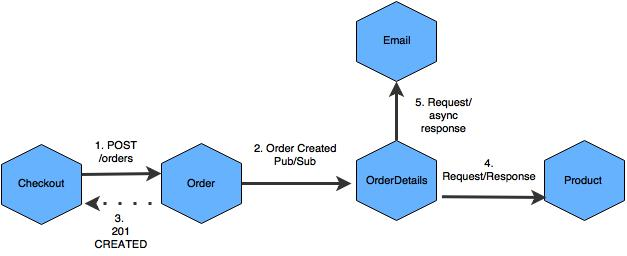
\includegraphics[width=0.8\textwidth]{figures/challanges_two_interaction_example}
\caption{Interaction during Order creation}
\label{fig:challanges_of_microservices_architecture/integration/inter_service_communication/interaction_during_order_creation}
\end{center}
\end{figure}
\\

\section{Distributed System Complexity}\label{section:challanges_of_microservices_architecture/distributed_system}
\subsection{Breaking Change}\label{section:challanges_of_microservices_architecture/integration/breaking_change}
\\
Although microservices are autonomous components, they still need to communicate. Also, it is obvious that they undergo changes frequently. However, some changes can be backward incompatible and break their consumers. The breaking changes are inevitable but however the impact of the breaking changes can be somehow reduced by applying various techniques. \cite{Newman:2015aa}
\begin{shaded}Techniques\end{shaded}
\begin{enumerate}
\item Avoid as much as possible \\ A good approach to reduce impact of incompatible changes to the consumers is to defer it as long as it is possible. One way is by choosing the correct integration technology such that loose coupling is maintained. For example, using \acrshort{REST} as an integration technology is better approach than using shared database because it encapsulates the underlying implementation and consumers are only tied to the interfaces.\\
Another approach is to apply TolerantReader pattern while accessing provider's \acrshort{API}. \cite{Fowler:2011aa} Consumer can get liberal while reading data from provider. Without blindly accepting everything from server, it can only filter the required data without caring about the payload structure and order. So, if the reader is tolerant, the consumer service can still work if the provider adds new fields or change the structure of the response.
\item Catch breaking changes early \\ It is also crucial to identify breaking change as soon as  possible when it happens. It can be achieved by using consumer-driven contracts. Consumers will write the contract to define the expectations from the producer's \acrshort{API} in the form of various integration tests. These integration tests can become a part of build process of the producer so the breaking change can be detected in the build process before the \acrshort{API} is accessed by the real consumers.
\item Use Semantic Versioning \\ Semantic Versioning is a way to identify the state of current artifact using compact information. It has the form MAJOR.MINOR.PATCH. MAJOR number is increased when backward incompatible changes are made. Similarly, MINOR number is increased when backward compatible functionalities are added. Finally, PATCH number represents that bug fixes are made which are backward compatible.\\
With semantic versioning, the consumers can clearly know if the provider's current update will break their \arshort{API} or not. For example, if consumer is using 1.1.3 version of provider's \arshort{API} and the new updated version is 2.1.3, then the consumer should expect some breaking changes and react accordingly.
\item Coexist Different Endpoints \\ Whenever a breaking change on a service is deployed, it should be carefully considered not to fail all the consumers immediately. One way is to support old version of end points as well as new ones. This will give some time for consumers to react on their side. Once all the consumers are upgraded to use new version of the provider, the old versioned end point can be removed. However, using this approach means that additional tests are required to verify both versions.
\item Coexist concurrent service versions \\ Another approach is to support both version of service at once. The requests from old consumers need to be routed to old versioned service and requests from new consumers to the new versioned service. It is mostly used when the cost of updating old consumer is high. However, this also means that two different versions have to be maintained and operated smoothly.
\end{enumerate}
\\
\begin{shaded}
At SAP Hybris, breaking change is avoided as much as possible using \acrshort{REST} and also Tolerant Reader pattern. When data is read from another microservice, the data is first handled by internal mapper library which maps the input data into the internal representation to be used by microservice. Also, for providing detailed information regarding state of current microservice version, semantic versioning is used. If there is breaking change in few endpoints, then multiple version of them is also maintained for short period of time giving the consumer fair amount of time to migrate. Similarly, if there are breaking changes in most of the endpoints then the entire microservice is maintained with different versions.
\end{shaded}
\subsection{Handling Failures}\label{section:challanges_of_microservices_architecture/handling_failures}
With a large number of microservices where communication is happening along not so reliable network, failures are inevitable. At the same time, it becomes challenging as well as highly necessary to handle the failures. Many strategies can be employed for the purpose. \cite{Newman:2015aa}\cite{Richardson:2015ab}\cite{Nygard:2007aa}
\begin{shaded}Techniques\end{shaded}
\begin{enumerate}
\item Timeouts \\ A service can get blocked indefinitely waiting for response from provider. To prevent this, a threshold value can be set for waiting. However, care should be taken not to choose very low or high value for waiting. 
\item Circuit Breaker \\ If request to a service keeps failing, there is no sense to keep sending request to the same server. It can be a better approach to track the request failures and stop sending further request to the service assuming that there is problem with the connection. By failing fast in such a way will not only save the waiting time for the client but also reduces unnecessary network load. Circuit Breaker pattern helps to accomplish the same. A circuit breaker has three states as shown in the Figure \ref{fig:challanges_of_microservices_architecture/integration/inter_service_communication/states_of_circuit_breaker}. In normal cases when the connection to the provider is working fine, it is in 'closed' state and all the connections to the provider goes through it. Once the connection starts failing and meets the threshold (can be number of failures or frequency of failures), the circuit breaker switch to 'open' state. At this state, any more connections fail straight away. After certain time interval, the state changes to 'half open' to check the state of provider again. Any connection request at this point passes through. If the connection is succesful, the state switches back to 'closed' state, else to 'open' state.\cite{Fowler:2014ac} \cite{Newman:2015aa} \cite{Nygard:2007aa}
\begin{figure}[H]
\begin{center}
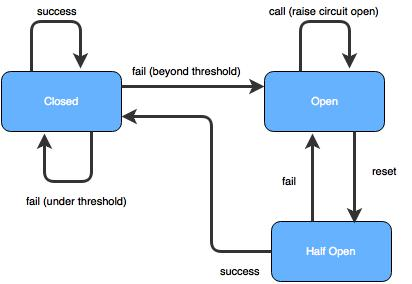
\includegraphics[width=0.8\textwidth]{figures/challanges_three_circuit_breaker}
\caption{States of a circuit breaker [\cite{Fowler:2014ac}]}
\label{fig:challanges_of_microservices_architecture/integration/inter_service_communication/states_of_circuit_breaker}
\end{center}
\end{figure}
\\
\item Bulk Head \\ Bulk Head is the approach of segregating various resources as per requirement and assigning them to respective purposes. Maintaining such threshold in available resources will save any resource from being constrained whenever there is problem in any section. One example of such bulkhead is the assignment of separate connection pool for each downstream resources. In this way, if problem in the request from one connection pool, it will not affect another connection pool and also not consume all available resources. \cite{Newman:2015aa} \cite{Nygard:2007aa}
\item Provide fallbacks \\ Various fallback logic can be applied along with timeout or circuit breaker to provide alternative mechanism to respond. For example, cached data or default value can be returned. 
\end{enumerate}
\\
\begin{shaded}
At SAP Hybris, synchronous requests are attempted recursively for certain number of times, each attempt waits for the response only for certain fixed amount of time depending upon usecase. In order to save network resources and provide fault tolerance, circuit breaker pattern is used.
\end{shaded}
\section{Operational Complexity}\label{section:challanges_of_microservices_architecture/operational_complexity}
\subsection{Monitoring}\label{section:challanges_of_microservices_architecture/monitoring}
With monolithic deployment, monitoring can be achieved by sifting through few logs on the server and looking various server metrics. The complexity can increase to some extent if the application is scaled along multiple server, in which case, monitoring can be performed by accumulating various server metrics and going through each log file on each host.
The complexity goes to whole new level when monitoring microservice deployment because of large number of individual log files produced by microservices. As difficult it is to go through each log files, it is even more challenging to trace any request contextually along all the log files.
\\
\begin{shaded}Techniques\end{shaded}
There are various ways to work around these complexities. \cite{Newman:2015aa} \cite{Simone:2014aa}
\begin{enumerate}
\item Log Aggregation and Visualition \\
A large number of logs in different locations can be intimidating. The tracing of logs can be easier if the logs could be aggregated in a centralized location and then visualized in a better way such as graphs. One of such variations can be achieved using ELK stack as shown in the Figure \ref{fig:challanges_of_microservices_architecture/elk_stack}. \cite{Anicas:2014aa} \cite{Newman:2015aa}
\begin{figure}[H]
\begin{center}
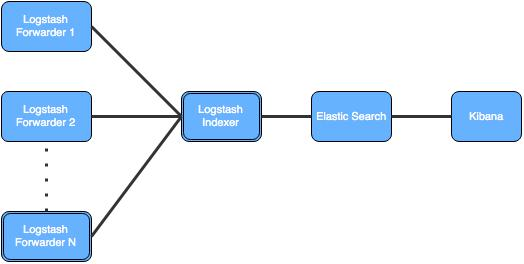
\includegraphics[width=0.8\textwidth]{figures/challenges_four_elk_stack}
\caption{ELK stack}
\label{fig:challanges_of_microservices_architecture/elk_stack}
\end{center}
\end{figure}
\\
The ELK stack consists of following major components.
\begin{enumerate}
\item Logstash Forwarder \\ It is the component installed in each node which forwards the selected log files to the central Logstash server.
\item Logstash Indexer \\ It is the central logstash component which gathers all the log files and process them.
\item Elastic Search \\ The Logstash Indexer forwards the log data and stores into Elastic Search.
\item Kibana \\ It provides web interface to search and visualize the log data.\\
The stack makes it easy to trace log and visualize graphs along various metrics.
\end{enumerate}
\item Synthetic Monitoring \\ Another aspect of monitoring which can be helpful, is to collect various health status such as availability, response time etc. There are many tools to make it easier. One such tool is 'uptime', which is a remote monitoring application and provides email notification as well as features such as webhook to notify a url using http POST.
\\
Rather than waiting for something to get wrong, a selected sets of important business logic can be tested in regular interval. The result can be fed into notification subsystem, which will trigger notification to responsible parties. This will ensure confidence that any problem will be detected as soon as possible and can be worked on sooner. \cite{Simone:2014aa} \cite{Newman:2015aa}
\item Correlation ID \\
A request from a client is fulfilled by a number of microservices, each microservice being responsible for certain part of the whole functionality. The request passes through various microservices until it succeeds. For this reason, it is difficult to track the request as well as visualize the complete logical path. 'Correlation ID' is an unique identification code assigned to the request by the microservice at the user end and passes it towards the downstream microservice. Each downstream microservice does the same and pass along the ID. It gets easier to capture a complete picture of any request in that way.
\end{enumerate}
\begin{shaded}
SAP Hybris uses ELK stack for monitoring and log visualization. In order to check the health status of microservices, 'uptime' tool is used. The webhook from the tool updates the central status page showing the current status of all the existing microservices. Any problem triggered by 'uptime' is also reflected in this page. Similary, a set of smoke tests are triggered from continuous integration tool such as TeamCity at regular interval. In order to track the requests at each microservices, a unique code is assigned to each request. The code is assigned by API-Proxy server which is the central gateway for any incoming request into \acrshort{YaaS}.
\end{shaded}

\subsection{Deployment}\label{section:challanges_of_microservices_architecture/deployment}
A major advantage of microservices is that the features can updated and delivered quickly due to the autonomity and independent deployability of each microservices. However, with the increase in the number of microservices and the rate of changes that can happen in each microservice, fast deployment is not straight forward. The culture of doing deployment for monolithic application will not work perfectly on microservices. This section discusses how it can be achieved.
\\
There are two major parts in deployment. In order to speed up deployment in microservices, approach to accomplish each part has to be changed slightly.
\begin{shaded}Techiniques\end{shaded}
\begin{enumerate}
\item Continuous Integration \\
It is a software development practice in which newly checked in code are followed by automated build and verification to ensure that the integration was successful. Following continuous integration does not only automate the artifact creation process but also reduces the feedback cycle of the code providing opportunity to improve quality.
\\
To ensure autonomy and agility in microservices, a better approach is to assign separate source code repository and separate build for each microservice as shown in Figure \ref{fig:challanges_of_microservices_architecture/deployment/continuous_integration}. Each repository is mapped to separate build in Continuous Integration server. Any changes in a microservice triggers corresponding build in Continuous Integration server and creates a single artifact for that microservice. An additional advantage of this approach is clear assignment of ownership of the repository and build responsibility to the teams, owning the microservices.  \cite{Newman:2015aa} \cite{Fowler:2006ab}
\begin{figure}[H]
\begin{center}
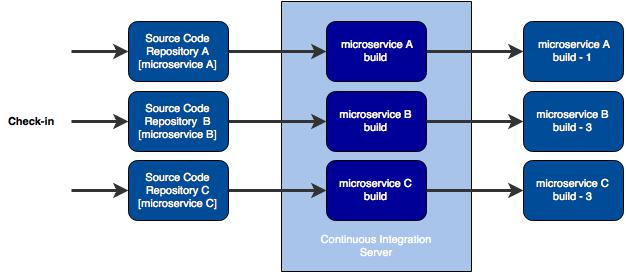
\includegraphics[width=0.8\textwidth]{figures/challenges_five_continuous_integration}
\caption{Continuous Integration \cite{Newman:2015aa}}
\label{fig:challanges_of_microservices_architecture/deployment/continuous_integration}
\end{center}
\end{figure}
\\
\item Continuous Delivery
\\
It is a discipline in which every small change is verified immediately to check deployability of the application. There are two major concepts associated with continuous deployment. First one is continuous integration of source code and creation of artifact. Next one is continuous deliver in which, the artifact is fed into a build pipeline. A build pipeline is a series of stages, each stage responsible for the verification of certain aspects of the artifact. A successful verification at each stage ensures the readiness of the artifact further close to release.
\\
\begin{figure}[H]
\begin{center}

\includegraphics[width=0.8\textwidth]{figures/challenges_six_continuous_delivery}
\caption{Continuous Delivery Pipeline \cite{Newman:2015aa}}
\label{fig:challanges_of_microservices_architecture/deployment/continuous_delivery}
\end{center}
\end{figure}
\\
A version of build pipeline is shown in Figure \ref{fig:challanges_of_microservices_architecture/deployment/continuous_delivery}. Here, faster tests are performed ahead and then slow tests, manual testing are performed down the line. This kind of successive verifications make it faster to identify problems, create clear visibility of problems and improve the quality as well as confidence in the quality of the application.\\
Each microservice has an independent build pipeline. The artifact build during continuous integration triggered by any change in the microservices is then fed into corresponding build pipeline for the microservice. \cite{Newman:2015aa} \cite{Fowler:2013aa}
\end{enumerate}

\begin{shaded}
The variation of continuous integration and deployment used at SAP Hybris is already discussed in Section \ref{section:hybris_architecture/deployment_workflow}.
\end{shaded}

\section{Conclusion}\label{section:challanges_of_microservices_architecture/conclusion}
In this chapter, various challenges needed to handle for assuring benefits from using microservices are listed. Each challenge is further broken down into fine constraints. Then, various ways of handling those constraints are discussed. Finally, the solution in the perspective of SAP Hybris is also presented. Microservices architecture provides efficient way to develop agile software however without a good grasp in the techniques to handle the challenges cannot be a good idea to start with microservice in the first place.













